

\chapter{Modelling of a rotating free-floating object dynamic interactions with a mass moving on its surface}
\label{ch:Stability study}
TOCHANGE!! purpose In this chapter is designing mass changes as control method one needs to establish the effect of changes of mass distributioon on a rotating free floating rotational motion and determine if there are and if so under what kind of conditions the motion of a mass at the surface of a free floating objects will imact its rotational motions
delpoyment of structure on frre floating object

define the stability of the rotational motion of the obejct???

System definition and model: The system is composed of an undeformable rotating object and a modular robot made out of identical spherical modules. The robots moves and deploys itself at the surface of the object by maintianing contact at all time. As the rotational motion is the only focus of this study, the system is considered to be isolated.
The best way to model is to use 

\section{Introductory illustration the Yo-Yo despin mechanism}
\label{Introductory illustration the Yo-Yo despin mechanism}

\subsection{System description}
drawing



Write..\gls{ghc}
Write..\gls{ghc}.


%\begin{figure}[h]
%	\begin{center}
%		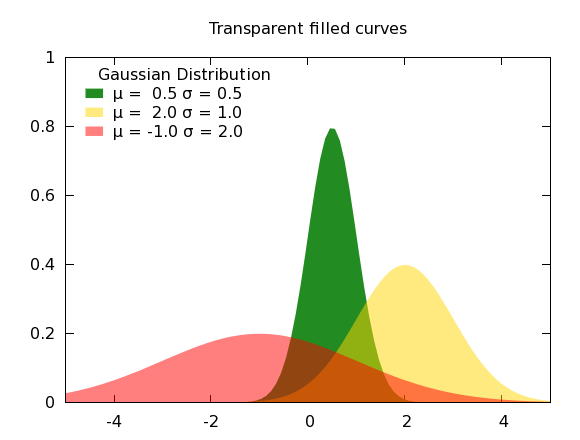
\includegraphics [width=12cm]{Figures/Background/pic.png}
%		\caption{Figure Caption.}
%		\label{fig:Yo-Yo despin mechanism seen in its plane of rotation}
%	\end{center}
%\end{figure} 



\section{System modelling}
\label{System modelling}
The Yo-Yo despin mechanism is discrete in order to generalise the robot and object were considered as a deformablee continuum where a rigid part (the object) would interact with a deformable part (the robot). The general model can be discrtized in order to accomodate the modular structure of the robot and simplify the dynamic equations of the system.

the model is directly derived from [PAPER]
\subsection{Continuous model}
\label{Continuous model}

As per [PAPER] the continuous model is the following: IN THE BODY FRAME
\begin{center}
\begin{equation*} 
\end{equation*}
\end{center}\
$[\bf I]\cdot \dot{\overrightarrow{\bf \Omega}} + \overrightarrow{\bf \Omega} \wedge [\bf I]\cdot \overrightarrow{\bf \Omega} + 2[\bf J]\cdot \overrightarrow{\bf \Omega}+ $

${d\over dt}{\int_{m}[(\overrightarrow{\bf \Psi} \otimes \overrightarrow{\bf x})\cdot \overrightarrow{\bf x} - (\overrightarrow{\bf x}\otimes\overrightarrow{\bf x})\cdot \overrightarrow{\bf \Psi}]dm}$



$+ \int_{m}{[(\overrightarrow{\bf x}\otimes \dot{\overrightarrow{\bf x''_{0}}}) - (\dot{\overrightarrow{\bf x''_{0}}}\otimes \overrightarrow{\bf x}) ]\cdot \overrightarrow{\bf \Psi}dm}$

$+\overrightarrow{\bf \Omega}\cdot \int_{m}{[(\overrightarrow{\bf x}\otimes \overrightarrow{\bf x})\wedge \overrightarrow{\bf \Psi}+((\overrightarrow{\bf x}\otimes \overrightarrow{\bf x})\wedge \overrightarrow{\bf \Psi})^{T}]dm}$

$\int_{m}(\overrightarrow{\bf x}\wedge \ddot{\overrightarrow{\bf x''_{0}}})
=\overrightarrow{\bf M}_{Body} + \overrightarrow{\bf M}_{Stresses}$




with $\overrightarrow{\bf \Omega}=\overrightarrow{\bf \Omega(t)}$ rigid body rotation constant over the continuum but depenmdent on time, $\overrightarrow{\bf \Psi}=\overrightarrow{\bf \Psi}(\overrightarrow{\bf x},t)$ dependent on the position whitihn the continuum and the time. 

$[\bf J]= \int_{m}{[(\overrightarrow{\bf v''_{0}} \cdot \overrightarrow{\bf x})[\bf 1] - \overrightarrow{\bf v''_{0}}\otimes \overrightarrow{\bf x}]dm}$.

Although model of a continuum, the interaction between mass(module) and the object does not constitute a stress hence $\overrightarrow{\bf M}_{Stresses}=\overrightarrow{\bf 0}$. Moreover the system is isolated so $\overrightarrow{\bf M}_{Body}=\overrightarrow{\bf 0}$.

\subsection{Discrete point mass model BEWARE IT NEGLECTS ROTATION ON Er AXIS IE ON ITSELF IN OTHER WORD THE ROTATION OF THE SPHERICAL BASIS ON ITSELF}
\label{Discrete point mass model}
For the purpose of studying the stability of the sytem will be studied with one moving mass along the surface of the object. This leads to the following discrete model:

$[\bf I]\cdot \dot{\overrightarrow{\bf \Omega}} + \overrightarrow{\bf \Omega} \wedge [\bf I]\cdot \overrightarrow{\bf \Omega}=$

$- 2m \big [(\dot{\overrightarrow{\bf x''_{0}}} \cdot \overrightarrow{\bf x})[\bf 1] - \dot{\overrightarrow{\bf x''_{0}}}\otimes \overrightarrow{\bf x}\big ]\cdot \overrightarrow{\bf \Omega}$

$-m \bigg [ \big [(\overrightarrow{\bf x} \cdot \overrightarrow{\bf x})[\bf 1]-(\overrightarrow{\bf x} \otimes \overrightarrow{\bf x}) \big] \cdot \dot{\overrightarrow{\bf \Psi}} + \big [2(\overrightarrow{\bf x}\cdot \dot{\overrightarrow{\bf x}})[\bf 1]-(\dot{\overrightarrow{\bf x}} \otimes \overrightarrow{\bf x})-(\overrightarrow{\bf x} \otimes \dot{\overrightarrow{\bf x}}) \big ]\cdot \overrightarrow{\bf \Psi} \bigg ]$

$-m{\big [(\overrightarrow{\bf x}\otimes \dot{\overrightarrow{\bf x''_{0}}}) - (\dot{\overrightarrow{\bf x''_{0}}}\otimes \overrightarrow{\bf x}) \big ]\cdot \overrightarrow{\bf \Psi}}$

$-m {\big [(\overrightarrow{\bf x}\otimes \overrightarrow{\bf x})\wedge \overrightarrow{\bf \Psi}+((\overrightarrow{\bf x}\otimes \overrightarrow{\bf x})\wedge \overrightarrow{\bf \Psi})^{T}\big ] \cdot \overrightarrow{\bf \Omega}}$

$-m(\overrightarrow{\bf x}\wedge \ddot{\overrightarrow{\bf x''_{0}}})$


Since the mass is bound to the surface the system is holonomic. Using the spherical cooordinates the relative kinematic properties of the mass with respect to the object can be expressed only with $\phi$ and $\theta$. The relative rotational speed and acceleration are respectively $\overrightarrow{\bf \Psi}= \begin{bmatrix}-sin(\phi)\dot \theta\\ cos(\phi) \dot \theta \\ \dot \phi  \end{bmatrix}$ and  $\dot{\overrightarrow{\bf\Psi}}=\begin{bmatrix}(-sin(\phi) \ddot \theta -cos(\phi) \dot \phi \dot \theta\\ cos(\phi) \ddot \theta -sin(\phi) \dot\phi \dot\theta\\ \ddot \phi)\end{bmatrix}$ as projected in the body frame.

The point hypothesis there is no additional rotation of the mass due to its following the surface (SEE DIAGRAM TO DRAW p58 my notebook). The local body coordiante system of the mass $[O'']$ can be considrerd to be the local shperical coordiante system. This leads to a the discrete model in body coordinate that will be used for our stability study:
$[\bf I]\cdot \dot{\overrightarrow{\bf \Omega}} + \overrightarrow{\bf \Omega} \wedge [\bf I]\cdot \overrightarrow{\bf \Omega}=m[\bf A]\cdot \overrightarrow{\bf \Omega}+m \overrightarrow{\bf R}$ where

$[\bf A]=\begin{bmatrix}
A_{1} & A_{2} & A_{3} \\ A_{4} & A_{5} & A_{6} \\ A_{7} & A_{8} & A_{9}
\end{bmatrix}$ and $\overrightarrow{\bf R}=\begin{bmatrix}
R1 \\R2 \\R3
\end{bmatrix}$

$A_{1}=2r \dot r (cos^2(\phi)sin^2(\theta)-1) - 2r^2 \dot \phi cos(\phi)sin(\phi)sin^2(\theta) +2r^2 \dot \theta cos^2(\phi)cos(\theta)sin(\theta)$

$A_{2}=A_{4}=2r \dot r cos(\phi)sin(\phi)sin^2(\theta)+r^2 \dot \phi sin^2(\theta)(cos^2(\phi)-sin^2(\phi))+2r^2 \dot \theta cos(\phi)sin(\phi)cos(\theta)sin(\theta)$

$A_{3}=A_{7}=2r \dot r cos(\phi)cos(\theta)sin(\theta) -r^2 \dot \phi sin(\phi)cos(\theta)sin(\theta)+r^2 \dot \theta cos(\phi)(cos^2(\theta)-sin^2(\theta))$

$A_{6}=A_{8}=2r \dot r sin(\phi)cos(\theta)sin(\theta) +r^2 \dot \phi cos(\phi)cos(\theta)sin(\theta)+r^2 \dot \theta sin(\phi)(cos^2(\theta)-sin^2(\theta))$

$A_{9}=-2r \dot r sin^2(\theta) - 2r^2 \dot \theta cos(\theta)sin(\theta)$

$R_{1}=r^2(cos(\phi)cos(\theta)sin(\theta) \ddot \phi+sin(\phi) \ddot \theta) +2r^2\dot \phi \dot \theta cos(\phi)cos^2(\theta)-r^2{\dot \phi}^2 sin(\phi)cos(\theta)sin(\theta)+ 2r\dot r (sin(\phi)\dot \theta+cos(\phi)cos(\theta)sin(\theta)\dot \phi)$

$R_{2}=r^2(sin(\phi)cos(\theta)sin(\theta) \ddot \phi-cos(\phi) \ddot \theta) +2r^2\dot \phi \dot \theta sin(\phi)cos^2(\theta)+r^2{\dot \phi}^2 cos(\phi)cos(\theta)sin(\theta)+ 2r\dot r (-cos(\phi)\dot \theta+sin(\phi)cos(\theta)sin(\theta)\dot \phi)$

$R_{3}=-r^2\ddot \phi sin^2(\theta)-2r^2\dot \theta \dot \phi cps(\theta)sin(\theta) -2r \dot r \dot \phi sin^2(\theta)$


 \glspl{pe}.

\section{Angular momentum and Energy Approach}
\label{Angular momentum and Energy Approach}
(all based on Tokis paper angular momentum and kinetic energy of rotating deformable bodies)
\subsection{Hypotheses}
TO FINISH!!!
EXACT CITATION FROM ARTICLE!!! p14 -16 cahier.
3 frames of reference:
Inertial Cartesian coordinate system centred at the CoM of the object $[O]\equiv (O, \vec{u_i}, \vec{x})$.

1) $\varepsilon$ Euclidian vector space with $\vec{u_i}$ basis vectors
E euclidian point space related to $\varepsilon$ and $\vec{x}$ position in $\varepsilon$ uniquely associated with a point $\vec{x}$ in E.

2) Rotating body Cartesian coordiante system with same origin O attached to the body to represent its rigid-body rotation $[O']\equiv (O, \vec{u_i'}, \vec{x'})$
$\vec{u_i'}$ time dependant base of $\varepsilon$
$\vec{x'}$ position in $\varepsilon$ uniquely assiociated with a point $\vec{x}$ in E wrt $\vec{u_i'}$.

The deformation in $[O']$ velocity and acceleration fields $\vec{v'}$ $\dot{\vec{v'}}$ expressed in $[O']$ with respect to $[O']$. (ie holding in $[O']$ when $[O']$ is stationary)

3) Cartesian coordiante system centred in O, $[O'']\equiv(O,\vec{u_i''}(x',t),\vec{x''})$ rotating relative to $[O']$ with a non-rigid body rotation. $\vec{u_i''(x',t)}$ position dependance in $[O']$ coordinates $\vec{x''}$ position in $\varepsilon$ of $\vec{x}$ in E but wrt $\vec{u_i''(x',t)}$ basis.

the reader is invited to read the paper for details
Each particle $(\vec{x'},t)$ can be regarded as possessing its own system $[O'']$ in which system and during its rotation the particle appears frozen. $[O'']$ is responsible for a rotation different from that of $[O']$ relativce to $[O]$.

Total rotational velocity is given as field $\vec{\Omega}(\vec{x},t)=\vec{\Omega}(t)+\vec{\Psi}(\vec{x},t)$
$\vec{\Omega}(\vec{x},t)$ angular velocity field in the total rotation of the configurations of the continuum B relative to the inertial frame $[O]$.
$\vec{\Omega}(t)$ spin of $[O']$ relative to $[O]$ rigid body rotation of continuum B.
$\vec{\Psi}(\vec{x},t)$ spin of $[O'']$ relative to $[O']$ expressed in inertial system $[O]$ and is the non-rigid body rotation of the configurations of the continuum B.
\subsection{Expression in any vector basis}
NOT CLEAR TO REVIEW!!!
A rotation is a linear application which conserves norms, angles, scalar, cross and dyadic products. In our case it is independant of the mass distribution meaning it can go from outside the integral to inside the integral.
Consequently, the following equations are valid and can be expressed in any basis at any point in time.

Position of the CoM: The CoM can be chosen to stay at O origin of inertial frame. In our model, there are no external forces and the no translation of the body in the inertial frame, therefore the CoM remains at the same place (you sse the deformation around a fixed CoM) TO REVIEW p21-22 cahier

In our model for all instant in time the body frame has its origin at the CoM. Threrefore, for every instant in time, we can project the equation on any basis we like. We can therefore chose to project the equation on the body axes which simplify our calculations ie principal axes of the body at any instant in time t.

\subsection{Objectives}
\subsubsection{Assumptions}
No friction the masses once in motion relative to the object wont require E in to carry on their motion and compensate dissipation.

The system object + mass is isolated there are no external forces or moments acting on the system =. this implies in the inertial frame conservation of the angular momentum ie $\vec{L_{inertial}}=\vec{constant}$.

The total energy of the system is also constant $T_{Total}=T_{Potential}+T_{Kinetic}=constant$.

\subsubsection{Engineering Objectives}
The objective is to maintain the rotational state of the object when the robot deploys.

Here we consider the system as going from an initial state to a state where the mass is attached (after landing) to a state where the mass is mouving due to a passive internal E transfer. The mass is allowed to move relative to the object. What i really mean here is that due to conservation of angular momentum the angular momentum just before and after relative motion starts is the sam irrespective of the reference frame (cte in inertial time dependent in body). Assuming instantaneous E transfer it occurs between mass and object since the system is isolated.

Objectives are two folds:

1) determine whether there exits a non-contributing angular momentum of the mass to the angular momentum of the system that would become the control command.

2) whether or under what resptrive hypotheses can a mass start moving and not affect the angular momentum of the object.

$T_{Potential}$ is stored inside the batteries of the robot otherwise there would be $T_{Kinetic}$ only.

\subsection{In our case}
(all based on Tokis paper angular momentum and kinetic energy of rotating deformable bodies)
Blending notation from the 2 papers:
$\bf [O_1]\equiv(O, \vec{x})$ inertial frame and $[\bf O_2]\equiv(O', \vec{y})$ non-rigid body rotation frame field dependent but centred on the same point $\bf O$ as the inertial frame which leads to the centre of $\bf [O_1]$ is the same as $\bf [O_2]$ hence $\overrightarrow{\bf x}=\overrightarrow{\bf x'}$. $\overrightarrow{\bf x'}$ is the position of a particle of the object in $[\bf O_2]$ but expressed in $[\bf O_1]$. $[\bf O_2]$ is a rotating spherical coordinate frame following the particle or mass in motion and from this perspective the mass moves only along $\overrightarrow{\bf e_r}$ and does not rotate in this frame. Also $\overrightarrow{\bf x}=\overrightarrow{\bf x'}=\overrightarrow{\bf e_r}$. At every time through a rotation, the equations can be expressed in any frame we want. The following equations can be expressed in the body frame with principal axes rigidly attached to the main ellipsoid object.

$\overrightarrow{\bf x}=[\bf A]*\overrightarrow{\bf y}$ with $[\bf A]$ change of frame between $[\bf O_1]$ and $[\bf O_2]$. 

$\dot{\overrightarrow{\bf x}}=\dot{\overrightarrow{\bf x'}}+\overrightarrow{\bf \Omega}(x,t)\wedge\overrightarrow{\bf x'}=\dot{\overrightarrow{\bf x'}}+\overrightarrow{\bf \Omega}(x,t)\wedge\overrightarrow{\bf x}$ since $\overrightarrow{\bf x}=\overrightarrow{\bf x'}$

$\dot{\overrightarrow{\bf x'}}$ velocity in $[\bf O_2]$ but expressed in $[\bf O_1]$ and eventually in body coordinates.
\subsubsection{Angular Momentum Calculation}
The angular momentum is an extensive quantity, a property that has been used to seperate the respective contributions of the object and the added mass.
Angular momentum calculated in inertial frame is 
$\overrightarrow{\bf L}^{[O_1]}=\int_{m}{[\overrightarrow{\bf x}\wedge\dot{\overrightarrow{\bf x}}]}dm$

$\overrightarrow{\bf L}^{[O_1]}=\int_{m}{[\overrightarrow{\bf x}\wedge(\dot{\overrightarrow{\bf x'}}+\overrightarrow{\bf \Omega}(x,t) \wedge \overrightarrow{\bf x})]}dm$

$\overrightarrow{\bf L}^{[O_1]}=\int_{m}{\overrightarrow{\bf x}\wedge\dot{\overrightarrow{\bf x'}}}dm+\int_{m}{\overrightarrow{\bf x}\wedge\ (\overrightarrow{\bf \Omega}(x,t) \wedge \overrightarrow{\bf x})}dm$

$\overrightarrow{\bf L}^{[O_1]}=\int_{m}{\overrightarrow{\bf x'}\wedge\dot{\overrightarrow{\bf x'}}}dm+\int_{m}{\overrightarrow{\bf x'}\wedge\ (\overrightarrow{\bf \Omega}(x,t) \wedge \overrightarrow{\bf x'})}dm$

$\overrightarrow{\bf L}^{[O_1]}=\int_{Body}{\overrightarrow{\bf x'}\wedge\dot{\overrightarrow{\bf x'}}}dm+\int_{Masses}{\overrightarrow{\bf x'}\wedge\dot{\overrightarrow{\bf x'}}}dm+\int_{Body}{\overrightarrow{\bf x'}\wedge\ (\overrightarrow{\bf \Omega}(x,t) \wedge \overrightarrow{\bf x'})}dm+\int_{Masses}{\overrightarrow{\bf x'}\wedge\ (\overrightarrow{\bf \Omega}(x,t) \wedge \overrightarrow{\bf x'})}dm$

$\overrightarrow{\bf L}^{[O_1]}=\overrightarrow{\bf L}^{[O_2]}_{Body}+\overrightarrow{\bf L}^{[O_2]}_{Masses}+\int_{Body}{\overrightarrow{\bf x'}\wedge\ (\overrightarrow{\bf \Omega}(x,t) \wedge \overrightarrow{\bf x'})}dm+\int_{Masses}{\overrightarrow{\bf x'}\wedge\ (\overrightarrow{\bf \Omega}(x,t) \wedge \overrightarrow{\bf x'})}dm$

In body coordinates using a spherical coordinates

$\overrightarrow{\bf x'}=r\overrightarrow{\bf e_r}$

$\dot{\overrightarrow{\bf x'}}=\dot{r}\overrightarrow{\bf e_r}$ deformation rate

$\int_{m}{\overrightarrow{\bf x'}\wedge\dot{\overrightarrow{\bf x'}}}dm=\int_{m}{r\overrightarrow{\bf e_r}\wedge\dot{r}\overrightarrow{\bf e_r}}dm=\overrightarrow{\bf 0}$

hence
$\overrightarrow{\bf L}^{[O_2]}_{Body}=\overrightarrow{\bf 0}$
$\overrightarrow{\bf L}^{[O_2]}_{Masses}=\overrightarrow{\bf 0}$

Finally

$\overrightarrow{\bf L}^{[O_1]}=\big[\bf I^{[O_1]}_{Body}\big] \overrightarrow{\bf \Omega}_{t} +m \big[r^2 [\bf Id]-\overrightarrow{\bf r}  \otimes \overrightarrow{\bf r} \big]\big(\overrightarrow{\bf \Omega}_{t}+\overrightarrow{\bf \Psi}(x,t)\big) $

cf paper for the trick
$\overrightarrow{\bf u} \wedge (\overrightarrow{\bf v} \wedge \overrightarrow{\bf w})=(\overrightarrow{\bf u} \cdot \overrightarrow{\bf w}) \overrightarrow{\bf v} - (\overrightarrow{\bf u} \cdot \overrightarrow{\bf v}) \overrightarrow{\bf w}$

$\overrightarrow{\bf x'}\wedge\ (\overrightarrow{\bf \Omega}_t \wedge \overrightarrow{\bf x'})=(\overrightarrow{\bf x'} \cdot \overrightarrow{\bf x'})\overrightarrow{\bf \Omega}_t - (\overrightarrow{\bf x'} \cdot \overrightarrow{\bf \Omega}_t)\overrightarrow{\bf x'}$

\subsubsection{Kinetic Energy Calculation}

$T=\frac{1}{2} \int_{m}{(\dot{\overrightarrow{\bf x}})^2dm}$

$T=\frac{1}{2} \int_{m}{\big (\dot{\overrightarrow{\bf x'}}+(\overrightarrow{\bf \Omega}(x,t) \wedge \overrightarrow{\bf x'})\big)^2dm}$ cf $\overrightarrow{\bf x}=\overrightarrow{\bf x'}$

$T=\frac{1}{2} \int_{m}{(\dot{\overrightarrow{\bf x'}})^2dm} +\frac{1}{2} \int_{m}{\big (\overrightarrow{\bf \Omega}(x,t) \wedge \overrightarrow{\bf x'}\big)^2dm}+\int_{m}{(\dot{\overrightarrow{\bf x'}} \cdot(\overrightarrow{\bf \Omega}(x,t) \wedge \overrightarrow{\bf x'}))dm}$ 

cf $\overrightarrow{\bf x}=\overrightarrow{\bf x'}$

But
$\frac{1}{2} \int_{m}{(\dot{\overrightarrow{\bf x'}})^2dm}=\frac{1}{2} \int_{Body+Masses}{(\dot{\overrightarrow{\bf x'}})^2dm}=\frac{1}{2} \int_{Masses}{(\dot{\overrightarrow{\bf x'}})^2dm}$ since the body is rigid. Moreover $\frac{1}{2} \int_{Masses}{(\dot{\overrightarrow{\bf x'}})^2dm}=\int_{Masses}{({\dot r \cdot \overrightarrow{\bf e_r}})^2dm}=\frac{m}{2}(\dot r)^2$ 

since it is relative velocity or deformation rate.

$\int_{m}{(\dot{\overrightarrow{\bf x'}} \cdot(\overrightarrow{\bf \Omega}(x,t) \wedge \overrightarrow{\bf x'}))dm}=\int_{m}{(\dot{r} \cdot \overrightarrow{\bf e_r} \cdot(\overrightarrow{\bf \Omega}(x,t) \wedge r \cdot \overrightarrow{\bf e_r}))dm}=\overrightarrow{\bf 0}$

$\int_{m}{(\overrightarrow{\bf \Omega}(x,t) \wedge \overrightarrow{\bf x'})\big)^2dm}=\int_{Body}{\big (\overrightarrow{\bf \Omega}_t \wedge \overrightarrow{\bf x'}\big)^2dm}+\int_{Masses}{\big (\overrightarrow{\bf \Omega}_t+\overrightarrow{\bf \Psi}(x,t) \wedge \overrightarrow{\bf x'}\big)^2dm}$

Finally
$T=\frac{m}{2}(\dot r)^2+\frac{1}{2}{\overrightarrow{\bf \Omega}_t}^T[\bf I^{[\bf O_1]=[\bf O_2]}]\overrightarrow{\bf \Omega}_t+\frac{m}{2}\big[(\overrightarrow{\bf \Omega}_t+\overrightarrow{\bf \Psi}(x,t)) \wedge r \cdot \overrightarrow{\bf e_r} \big ]^2$

$T=\frac{m}{2}(\dot r)^2+\frac{1}{2}{\overrightarrow{\bf \Omega}_t}^T[\bf I^{[\bf O_1]=[\bf O_2]}]\overrightarrow{\bf \Omega}_t+\frac{m}{2}\big(\overrightarrow{\bf \Omega}_t+\overrightarrow{\bf \Psi}(x,t)\big)^T\big[r^2 [\bf Id]-\overrightarrow{\bf r}  \otimes \overrightarrow{\bf r} \big]\big(\overrightarrow{\bf \Omega}_t+\overrightarrow{\bf \Psi}(x,t)\big) $

We will use this in the rigid body frame.

Dyadic product porperty $(\underline{\bf C} \wedge \bf A) \cdot \underline{\bf D} =\underline{\bf C} \cdot (\bf A \wedge \underline{\bf D})$

$\otimes$
Write.. \gls{pe}.

Write.. \glspl{pe}.

\section{Angular Velocity Command}
\label{Angular Velocity Command}
angular momentum at t=0
$\overrightarrow{\bf L}^{[O_1]}=\big[\bf I^{[O_1]}_{Body}\big] \overrightarrow{\bf \Omega}_{t} +\big [I_{Mass}(x,t)\big] \big(\overrightarrow{\bf \Omega}_{t}+\overrightarrow{\bf \Psi}(x,t)\big)= \big(\big[\bf I^{[O_1]}_{Body}\big] +\big [I_{Mass}(x,t)\big]\big) \overrightarrow{\bf \Omega}_{t}+\big [I_{Mass}(x,t)\big]\overrightarrow{\bf \Psi}(x,t)$

where $\big[ \bf I_{Mass}(x,t) \big]=m \big[r^2 [\bf Id]-\overrightarrow{\bf r}  \otimes \overrightarrow{\bf r} \big]$

\subsection{Non contributing velocity command}
\label{Non contributing velocity command}
$\big[ \bf I_{Mass}(x,t) \big]=\begin{bmatrix}
1 - cos(\phi)^2sin(\theta)^2 & -sin(\phi)cos(\phi)sin(\theta)^2 & -cos(\theta)cos(\phi)sin(\theta) \\ -cos(\phi)sin(\phi)sin(\theta)^2 & 1 - sin(\phi)^2sin(\theta)^2 & -cos(\theta)sin(\phi)sin(\theta) \\ -cos(\phi)sin(\theta)cos(\theta) & -sin(\phi)sin(\theta)cos(\theta) & sin(\theta)^2
\end{bmatrix}$

$det(\big[ \bf {I_{Mass}(x,t)} \big])=1 - cos(\phi)^2*sin(\theta)^2 - sin(\phi)^2*sin(\theta)^2 - cos(\theta)^2 
=  sin(\theta)^2 -  sin(\theta)^2*(cos(\phi)^2+sin(\phi)^2) = 0$

the instantaneous eigenvalues of $\big[ \bf {I_{Mass}(x,t)} \big]$ are $1$, $1$ and $1 - cos(\phi)^2*sin(\theta)^2 - sin(\phi)^2*sin(\theta)^2 - cos(\theta)^2=0$ its rank is therefore $2$ at any given time.

This does mean that we can prescribe a velocity command that does not contribute directly to the overall angular momentum only by a time dependant component of the moment of inertia whose ratio with the object moment of inertia is to be determined to have a small effect as follows:
If $$\big[ \bf {I_{Mass}(x,t)} \big]=\begin{bmatrix}
	I_{1} & I_{2} & I_{3} \\ I_{4} & I_{5} & I_{6} \\ I_{7} & I_{8} & I_{9}
\end{bmatrix}$$
then $\overrightarrow{\bf \Psi}(x,t)$ can be prescribed as follows
$\overrightarrow{\bf \Psi}(x,t)=\begin{bmatrix}
-\begin{bmatrix}I_{1} & I_{2}  \\ I_{4} & I_{5}\end{bmatrix}^{-1} \begin{bmatrix} I_{3}\\ I_{6}\end{bmatrix}  \\ 1
\end{bmatrix}*\Psi_z=\begin{bmatrix}
cos(\phi)*tan(\theta) \\
sin(\phi)*tan(\theta) \\ 1 \end{bmatrix}*\Psi_z=>\begin{bmatrix}
cos(\phi)*sin(\theta) \\sin(\phi)*sin(\theta) \\ cos(\theta) \end{bmatrix}*\Psi_z$ where $\Psi_z$ can be any function (to eliminate side effect due to division to 0 by keeping proportionality). It can be easily verified that
$\big [\bf I_{Mass}(x,t)\big]\overrightarrow{\bf \Psi}(x,t)=\overrightarrow{\bf 0}$ but also it is obvious from the fact that it is $\Psi_z*\overrightarrow{\bf x}$ instantaneous rotation about the radial component which does not contribute to the overall angular momentum ROTATION ON ITSELF CANNOT BE NEGLECTED HOW TO LINK TO SPHERICAL COORDINATES TO PICTURE A TRAJECTORY. PLUS POINT MASS MODEL IS WRONG SINCE THE SPHERICAL BASIS ROTATE ONITSELF ON ITS R AXIS SPHERICAL BASIS CANNOT DECRIBE THIS AS THE BASIS IS ROTATING ON ITRSELF

As per [CHENG SPHERICAL ROTATION COORDINATE SYSTEM] paper the angle describing pure rotation about the instantaneous radius vector/axis is independent from polar and azimuthal angles meaning it can vary independalty. Therefore pure rotation about the radial axis generated by the radial vecto as defined in spherical coordiantes cannot be described with the polar and azimuthal angles reporting the position of the mass on the spherical sphere of radius 1. there cannot be an angular velocity command which does not contribute (FIND A BETTER TERM) to the overall angular momentum.

At any one time the first 2 rows combine into the third with the coefficient $lambda =\begin{bmatrix}
-cos(\phi)*tan(\theta) \\
-sin(\phi)*tan(\theta)
\end{bmatrix} => \begin{bmatrix}
row 1 \\row 2
\end{bmatrix}$

\subsection{Error vector magnitude stability?}
\label{Error vector magnitude stability?}
The angular momentum remains:
$ \Big(\big[\bf I^{[O_1]}_{Body}\big] +\big [I_{Mass}(x,t)\big]\Big) \overrightarrow{\bf \Omega}_{t}+\big [I_{Mass}(x,t)\big]\overrightarrow{\bf \Psi}(x,t)$
It is assumed that $M_{Object}>>M_{module}$ and that there is an E transfer between potential E of the battery and the mass or module, but the E transferred given the mass ration is negligible enough so as to not alter the angular momentum which is still conserved between the instant when the mass is attached to the instant it starts mouving relative to the object.

$ \Big(\big[\bf I^{[O_1]}_{Body}\big] +\big [I_{Mass}(x_0,t_0)\big]\Big) \overrightarrow{\bf \Omega}^{0}_{t}= \Big(\big[\bf I^{[O_1]}_{Body}\big] +\big [I_{Mass}(x,t)\big]\Big) \overrightarrow{\bf \Omega}^{1}_{t}+\big [I_{Mass}(x,t)\big]\overrightarrow{\bf \Psi}(x,t)$

Introducing the error vector $\overrightarrow{\bf \epsilon}_{t}$ such that $\overrightarrow{\bf \Omega}^{1}_{t}=\overrightarrow{\bf \Omega}^{0}_{t}+\overrightarrow{\bf \epsilon}_{t}$

$\overrightarrow{\bf \varepsilon}_{t}=\Big(\big[\bf I^{[O_1]}_{Body}\big] +\big [I_{Mass}(x,t)\big]\Big)^{-1}\bigg(\big(\big [I_{Mass}(x_0,t_0)\big]-\big [I_{Mass}(x,t)\big]\big) \overrightarrow{\bf \Omega}^{0}_{t}-\big [I_{Mass}(x,t)\big]\overrightarrow{\bf \Psi}(x,t) \bigg)$
\subsection{Elimination of the added mass}
\label{Elimination of the added mass}
when psi=-omega
\subsubsection{naive control command opposite velocity}
\label{opposite velocity}
the idea here is that the mass counteracts perfectly the angular velocity of the object when attached so that it appears to go in the opppsoite direction. In the inertial frame the mass will be immobile and the system will behave as if no mass is on the surface of the object. This would garanty that we can derive the motion of the objec providing initial conditions are known. The mass reease will influence those itnial conditions

Problem is since the motion of thje object is periodic the curve described by the mass on the surface will be a closed curve and it will follow a path dependend on the angular velocity and the lending site which means it wont cover the surface not to mention that if the anguklar velocity's magnitude is large the robot may not have the capabilitites to follow. Also depending on the landing site the initail conditions may be the wrong ones. landing sitre may be optimal in sense of conserving angular velocity prior to landing but not when the mass is realese in terms of initial conditions. NEED LANDING SITE FIRST

\subsection{Landing site}
\label{Landing site}
\subsubsection{Ellipsoid generation}

$a > b > c$ - general or tri-axial ellipsoid

$a = b > c$ - oblate ellipsoid of revolution (or oblate spheroid)

$a = b < c$ - prolate ellipsoid of revolution (or prolate spheroid)

$a = b = c$ - sphere (often referred to as the degenerate case)

Sidi: maximum inertia is major axis minimum inertia is minor axis.

Moment of inertia of an ellipsoid
$A=\frac{1}{5}(b^2+c^2)$ along $a$ or $x$ axis
$B=\frac{1}{5}(a^2+c^2)$ along $b$ or $y$ axis
$C=\frac{1}{5}(a^2+b^2)$ along $c$ or $z$ axis
Evidently we have
$c \geq a,b \Rightarrow I_{xx}, I_{yy} \geq I_{zz}$ the longest axis (shortest axis) has the smallest (largest) moment of inertia repectively.




Error = for theta=0

-(B + 1)*Cx/(1+ A + B + A*B) 

-(A+ 1)*Cy /(1  + A + B + A*B) ~ mr2

-(  0)/(C + A*C + B*C + A*B*C )=0 => landing on the tip seems ok but if it is woobly difficlt to land best for spinning object (ie near symmetrical?)


$Radius=c^2$ c always the longest and minor(to check) axis

can we safely assume that there are no transfer of E look up added mass model RATIO

does not depend on added mass FALSE
if you land at the tip no influence on the “spinning” axis for near symmetric bodies TRUE


evolution of percentage for different angles

\subsubsection{Model}
\label{Model}
The choice for the landing site is dependent on the disturbance it generates to the rotational motion of the object. The best landing site should therefore generate minimum disturbance. It is important because it is one of the parameters of the error vector when the mass is mouving along the surface as one of its initial conditions. The motion of the mass will generate its own disturbances and it is important to  minimise the overall contribution of all htes e disturbances.

According to [Dynamics of Bodies with variable mass by Cveticanin] the angular momentum for body addition is as calculated at the origin of our different frames of referenc ie the CoM of the object. Since the addition of mass is symmetric with respect to the CoM of the object the calculations are valid since CoM $O$ does not move between object and object plus added mass

$\Delta \overrightarrow{\bf L}_{O}= \overrightarrow{\bf L}_{S1}-\overrightarrow{\bf L}_{S2}-\overrightarrow{\bf L}_{S}+\overrightarrow{\bf \rho_{S2}}\wedge mass*\big(\overrightarrow{\bf v}_{S1}-\overrightarrow{\bf v}_{S2} \big)=[\bf I_{S1}\big]\overrightarrow{\bf \Omega}_{S1}-[\bf I_{S2}\big]\overrightarrow{\bf \Omega}_{S2}-[\bf I_{S}\big]\overrightarrow{\bf \Omega}_{S}+\overrightarrow{\bf \rho_{S2}}\wedge mass*\big(\overrightarrow{\bf v}_{S1}-\overrightarrow{\bf v}_{S2} \big)$

where $\overrightarrow{\bf L}_{S}$ is the angular momentum of the initial body with respect to its CoM, $\overrightarrow{\bf L}_{S2}$ is the angiular momentum of the added mass prior to addition wrt its own CoM and  $\overrightarrow{\bf L}_{S1}$ is the angular momentum of the final body woith respect to its new CoM. $\overrightarrow{\bf \rho}_{S2}$ is the vector between the CoM of the object and the CoM of the added mass. and then the relative velocity between the two objects.


Quote:"According to the principle of linear momentum, variation of the momentum for discontinula mass addition in time interval $\Delta t$ is equal to the impulse $\overrightarrow{\bf J}^{\bf F-r}$ of the resultant force $\overrightarrow{\bf F_r}$ of all external active forces and constraint reactions $\overrightarrow{\bf F_r}=Mass*\big(\overrightarrow{\bf v}_{S1}-\overrightarrow{\bf v}_{S}\big)+mass*\big(\overrightarrow{\bf v}_{S1}-\overrightarrow{\bf v}_{S2}\big)$"


Quote: "The variation of the angular momentum in the time interval $\Delta t$ is equalt to the impulse $\overrightarrow{\bf J}^{\bf M}$ which is the sum of the impulse fo the moment of the resultant force $\overrightarrow{\bf M}_{\bf O}^{\bf F_r}$ for point $O$ and the impulse of the resultant torque $\overrightarrow{\bf M}$ caused by active torque and constraint reaction torque during mass addition."

then

$\overrightarrow{\bf L}_{S1}-\overrightarrow{\bf L}_{S2}-\overrightarrow{\bf L}_{S}+\overrightarrow{\bf \rho_{S1}}\wedge (Mass+mass)*\overrightarrow{\bf v}_{S1}-mass*\overrightarrow{\bf \rho_{S2}}\wedge\overrightarrow{\bf v}_{S2}=\overrightarrow{\bf J}^{\bf M}$

where $\overrightarrow{\bf J}^{\bf M}=\big(\overrightarrow{\bf M}_{\bf O}^{\bf F_r}+\overrightarrow{\bf M}\big) \Delta t$

Quote:"If impulses of external forces $\overrightarrow{\bf J}^{\bf F_r}$ and torques $\overrightarrow{\bf J}^{\bf M}$ are quite small, due to short time $\Delta t$, system is assumed to be without action of external forces and torques. In that case variation of the angular momnetum is $\Delta \overrightarrow{\bf L}_{O}=\overrightarrow{\bf 0}$ ie angular momentums of the system before and after mass variation remains invariable."

hence

$\overrightarrow{\bf L}_{S1}=\overrightarrow{\bf L}_{S2}+\overrightarrow{\bf L}_{S}-\overrightarrow{\bf \rho_{S1}}\wedge (Mass+mass)*\overrightarrow{\bf v}_{S1}+mass*\overrightarrow{\bf \rho_{S2}}\wedge\overrightarrow{\bf v}_{S2}$

Finally

$[\bf I_{S1}\big]\overrightarrow{\bf \Omega}_{S1}=[\bf I_{S2}\big]\overrightarrow{\bf \Omega}_{S2}+[\bf I_{S}\big]\overrightarrow{\bf \Omega}_{S}-\overrightarrow{\bf \rho_{S2}}\wedge mass*\big(\overrightarrow{\bf v}_{S1}-\overrightarrow{\bf v}_{S2} \big)$

Our assumptions:
\begin{itemize}
	\item there are no exrternal forces on system Object+added mass but quid resultant torque
	\item point mass which leads $\overrightarrow{\bf L}_{S2}=\overrightarrow{\bf 0}$
	\item since we are concerned solely with angular rotation ther is no object velocity inthe inertial frame $\overrightarrow{\bf v}_{S1}=\overrightarrow{\bf 0}$
	\item we assume that in the last phase of approach of the robot before landing the robot follows the rotational motion
\end{itemize} 
\begin{itemize}
	\item $Mass \gg mass$
	\item OR addition of mass is symmetric in space but we same velocity
\end{itemize}

we have $\overrightarrow{\bf L}_{S1}=\overrightarrow{\bf L}_{S}+mass*\overrightarrow{\bf \rho_{S2}}\wedge\overrightarrow{\bf v}_{S2}$

first point $mass*\overrightarrow{\bf \rho_{S2}}\wedge\overrightarrow{\bf v}_{S2} \approx \overrightarrow{\bf 0}$

second point $\frac{mass}{2}*\overrightarrow{\bf \rho_{S2}}\wedge\overrightarrow{\bf v}_{S2}+\frac{mass}{2}*-\overrightarrow{\bf \rho_{S2}}\wedge\overrightarrow{\bf v}_{S2} = \overrightarrow{\bf 0}$

third point we can consider that the mass does not rotate on itself if it is modelled as a sphere and has a translational rotational motion (like the earth).


\subsubsection{Error vector}
The addition of mass whether point 1 or 2 above will alter the angular velocity to an extent either by pure mass addition or by mass addition + the relative angular momentum due to the relative velocity at impact. All of these effect are modelled by an error vector added to the original angular velocity. we are going to investigate later what are the impact over time of this error ie magnitude anfg frequencey (not quite the right terms)

$ \Big(\big[\bf I^{[O_1]}_{Body}\big] +\big [I_{Mass}(x_1,t_1)\big]\Big) \overrightarrow{\bf \Omega}^{1}_{t}= \big[\bf I^{[O_1]}_{Body}\big]\overrightarrow{\bf \Omega}^{0}_{t}$

Introducing the error vector $\overrightarrow{\bf \epsilon}_{t}$ such that $\overrightarrow{\bf \Omega}^{1}_{t}=\overrightarrow{\bf \Omega}^{0}_{t}+\overrightarrow{\bf \epsilon}_{t}$

$\overrightarrow{\bf \varepsilon}_{t}=-\bigg(\big[\bf I^{[O_1]}_{Body}\big] +\big [I_{Mass}(x_1,t_1)\big]\bigg)^{-1}\bigg(\big [I_{Mass}(x_1,t_1)\big] \overrightarrow{\bf \Omega}^{0}_{t} \bigg)$

Erro to the kinetic energy

$2T_{1}={\overrightarrow{\bf \Omega}^{1}_{t}}^{T} \Big(\big[\bf I^{[O_1]}_{Body}\big] +\big [I_{Mass}(x_1,t_1)\big]\Big) \overrightarrow{\bf \Omega}^{1}_{t}$

given what we have for the angualr momnetum just above

$2T_{1}=(\overrightarrow{\bf \Omega}^{0}_{t}+\overrightarrow \epsilon_{t})^{T} \Big(\big[\bf I^{[O_1]}_{Body}\big]\Big) \overrightarrow{\bf \Omega}^{0}_{t}=2T_{0}+ \overrightarrow \epsilon_{t} \cdot \overrightarrow{\bf \Omega}^{0}_{t}$

hence
%\begin{equation}
$$ T_{error}=\frac{1}{2}\Delta T= -\frac{1}{2} \bigg(\big[\bf I^{[O_1]}_{Body}\big] +\big [I_{Mass}(x_1,t_1)\big]\bigg)^{-1}\bigg(\big [I_{Mass}(x_1,t_1)\big] \overrightarrow{\bf \Omega}^{0}_{t} \bigg) \cdot \Big(\big[\bf I^{[O_1]}_{Body}\big]\Big) \overrightarrow{\bf \Omega}^{0}_{t} $$
%\end{equation}

Everything is dependent on $\overrightarrow{\bf \Omega}^{0}_{t}$ for which we can use the genral soolution to have the boundaries between which its magnitude and the magnitude of its components vary.


General solutions of the Euler equations:

$\omega_{x}=\sqrt{\frac{h^2 - 2TC}{A(A-C)}} elliptic fct=\sqrt{2T}\sqrt{\frac{\frac{h^2}{2T} - C}{A(A-C)}} elliptic fct$ TODO ELLIPTIC FUNCTION

$\omega_{y}=\sqrt{\frac{h^2 - 2TC}{B(B-C)}} elliptic fct=\sqrt{2T}\sqrt{\frac{\frac{h^2}{2T} - C}{B(B-C)}} elliptic fct$

$\omega_{z}=\sqrt{\frac{2TA - h^2}{C(A-C)}} elliptic fct=\sqrt{2T}\sqrt{\frac{A - \frac{h^2}{2T}}{C(A-C)}} elliptic fct$

We take the upper bound of these for this study

Regarding the parameters composing the function:
\begin{itemize}
	\item $A,B,C=fct(a,b,c)$ where $a,b,c$ are normalised
	\item $\frac{h}{2T}=cte$ and $\frac{h}{2T} \in [\min(A,B,C), \max(A,B,C)]$. Our choice if $\min(A,B,C)=\alpha$ and $\max(A,B,C)=\beta$ then we choose this list $\frac{h}{2T} \in \{\alpha, \frac{3\alpha+\beta}{4}, \frac{\alpha+\beta}{2}, \frac{\alpha + 3\beta}{4}, \beta\}$
	\item the mass of the robot is normalised to $m=1$, we can therefore use the mass ratio $MR$ directly to simulate the mass of the object. The density which is an important parameter for realistic object varies implicitly
	\item but we need a value for the kinetic energy $T$ which in general $T=\frac{1}{2}{\overrightarrow{\bf \Omega}^{0}_{t}}^{T}\begin{bmatrix}
	A&0&0\\0&B&0\\0&0&C
	\end{bmatrix}\overrightarrow{\bf \Omega}^{0}_{t}$ and depends on the shape of the ellipsoid ie paramters $a,b,c$
\end{itemize}


In order to calculate $T$ in the general case we need to know what are the components of the angular velocity. However these components are what we are trying to calculate in the first place but given the solutions to Euler equations. As per below we can choose the magnitude of the rotational speed according to what can be found in space (see below PERHAPS A RANGE WOULD BE GOOD FOR CONTROL COMMAND). SINCE WE CONSIDER MASS AS POINT MASS WE CAN NORMALISE THE DIMENSIONS OF THE ELLIPSOID ie $a,b,c$ BECAUSE NOTHING REALLY DEPENDS ON THE RELATIVE DIMENSION BETWEEN THE 2 ONLY THE RELATIVE MASS, THE ADDED MASS IS CONTRAINED BY AN HOLONOMIC LINK. One easy compromise is to use a sphere since the knowledge of the magnitude of the angular velocity is enough as all moments of inertia are equal as well as all the parameters (NAME). Hence $2T=Aw^2=\frac{1}{5}(b^2+c^2)Mass*w^2=\frac{1}{5}(1^2+1^2)MassRatio*w^2=\frac{2}{5}MassRatio*w^2$ and this will be calculated for each ellipsoid!


As per "Asteroid mining 101" p39 we take a mid range composition of a stony-irons asteroid of density $5500 kg/m^3$ p116 majority of NEAs are less than $100 m$ in diameter and have rotation periods of a few minutes we choose 5min ie $0.020943951023932 rad.s^{-1}$. This gives a magnitude for the energy of $T=40.42299774616883 GJ$ Solid sphere of radius r and mass m has $I=\frac{2}{5}mr^2$ volume of sphere $V=\frac{4}{3}\pi r^3$. mass $m=2.303834612632515e+10kg$.
\subsection{System plant time-dependent state space model}
$ \Big(\big[\bf I^{[O_1]}_{Body}\big] +\big [I_{Mass}(x_1,t_1)\big]\Big) \overrightarrow{\bf \Omega}^{1}_{t}+\big [I_{Mass}(x_1,t_1)\big] \overrightarrow{\bf \Psi}(x,t)= \Big(\big[\bf I^{[O_1]}_{Body}\big] +\big [I_{Mass}(x_0,t_0)\big]\Big)\overrightarrow{\bf \Omega}^{0}_{t}$

Introducing the error vector $\overrightarrow{\bf \epsilon}_{t}$ such that $\overrightarrow{\bf \Omega}^{1}_{t}=\overrightarrow{\bf \Omega}^{0}_{t}+\overrightarrow{\bf \epsilon}_{t}$

$\overrightarrow{\bf \varepsilon}_{t}=\bigg(\big[\bf I^{[O_1]}_{Body}\big] +\big [I_{Mass}(x_1,t_1)\big]\bigg)^{-1}\bigg(\Big(\big [I_{Mass}(x_0,t_0)\big]-\big [I_{Mass}(x_1,t_1)\big] \Big) \overrightarrow{\bf \Omega}^{0}_{t} -\big [I_{Mass}(x_1,t_1)\big] \overrightarrow{\bf \Psi}(x,t)\bigg)$

\subsubsection{System equilibria USEFUL??}
\label{System equilibrian}

In [BOOK] the sytem is nonautonomous of the form $\dot x =f(x,t)$ and what we are interested in is the equilibrium for the object i.e. $\dot{ \overrightarrow{\bf \Omega}}=\overrightarrow{\bf 0}$. the componenets with the angles are the time dependent part

Euler equation for rigid body $\dot{ \overrightarrow{\Omega}}=\dot {\overrightarrow{0}} =>$

$\omega_{y}\omega_{z}(I_{z}-I_{y})=0$

$\omega_{x}\omega_{z}(I_{x}-I_{z})=0$

$\omega_{x}\omega_{y}(I_{z}-I_{y})=0$

This implies that at least two of these angular velocities are null, meaning we are in pure constant spin. but most rotational state are described by the solutions of the Euler equations and therefore this is what we have to maintain so equilibria study is not relevant.
\subsubsection{Observability and controllability}
\subsubsection{Design of a MPC feedback controller for maintaining the initial rotational state (with  and without constraints)}
\subsubsection{Design of a MPC feedback controller for controlling the rotational state of the object (with  and without constraints)}




